% ============================================================
% Diagram: Structure of Indian Boundary Hierarchies
% Compile with: pdflatex diagram_boundary_hierarchy.tex
% Requires: tikz, tikzlibrary{shapes,arrows.meta,positioning,fit,backgrounds,calc}
% ============================================================
\documentclass[tikz, border=12pt]{standalone}
\usepackage{tikz}
\usepackage{xcolor}
\usetikzlibrary{shapes.geometric, arrows.meta, positioning, fit, backgrounds, calc}

% ── Colour palette ────────────────────────────────────────────────────────────
\definecolor{admblue}{RGB}{210,228,255}
\definecolor{admborder}{RGB}{50,90,170}
\definecolor{elecred}{RGB}{255,215,210}
\definecolor{elecborder}{RGB}{170,50,40}
\definecolor{fegreen}{RGB}{210,245,220}
\definecolor{fegreenborder}{RGB}{40,140,70}
\definecolor{overlayyellow}{RGB}{255,248,200}
\definecolor{overlayborder}{RGB}{180,140,0}
\definecolor{gpbox}{RGB}{225,210,255}
\definecolor{gpborder}{RGB}{90,50,170}
\definecolor{notegrey}{RGB}{245,245,245}
\definecolor{annotgrey}{RGB}{90,90,90}
\definecolor{containarrow}{RGB}{50,90,170}
\definecolor{overlaparrow}{RGB}{200,100,0}

\tikzset{
  admbox/.style  = {draw=admborder,    fill=admblue,   rounded corners=5pt,
                    minimum width=4.8cm, align=center, font=\small,
                    inner sep=7pt, minimum height=1.1cm},
  elecbox/.style = {draw=elecborder,   fill=elecred,   rounded corners=5pt,
                    minimum width=4.8cm, align=center, font=\small,
                    inner sep=7pt, minimum height=1.1cm},
  gpbox/.style   = {draw=gpborder,     fill=gpbox,     rounded corners=5pt,
                    minimum width=4.8cm, align=center, font=\small,
                    inner sep=7pt, minimum height=1.1cm},
  febox/.style   = {draw=fegreenborder,fill=fegreen,   rounded corners=5pt,
                    minimum width=10.8cm, align=center, font=\small,
                    inner sep=8pt, minimum height=1.1cm},
  overlaybox/.style={draw=overlayborder,fill=overlayyellow, rounded corners=5pt,
                    minimum width=10.8cm, align=center, font=\small,
                    inner sep=7pt, minimum height=1.0cm},
  notebox/.style = {draw=black!25,     fill=notegrey,  rounded corners=3pt,
                    minimum width=4.8cm, align=left, font=\footnotesize,
                    inner sep=6pt},
  containarrow/.style = {-{Latex[length=2.5mm]}, thick, color=containarrow,
                          shorten >=1pt, shorten <=1pt},
  overlaparrow/.style = {-{Latex[length=2.5mm]}, dashed, thick, color=overlaparrow,
                          shorten >=1pt, shorten <=1pt},
  bracelab/.style= {font=\footnotesize\itshape, color=annotgrey},
  seclabel/.style= {font=\small\bfseries, inner sep=4pt},
  legend/.style  = {draw=black!30, fill=white, rounded corners=3pt,
                    inner sep=8pt, font=\footnotesize}
}

\begin{document}
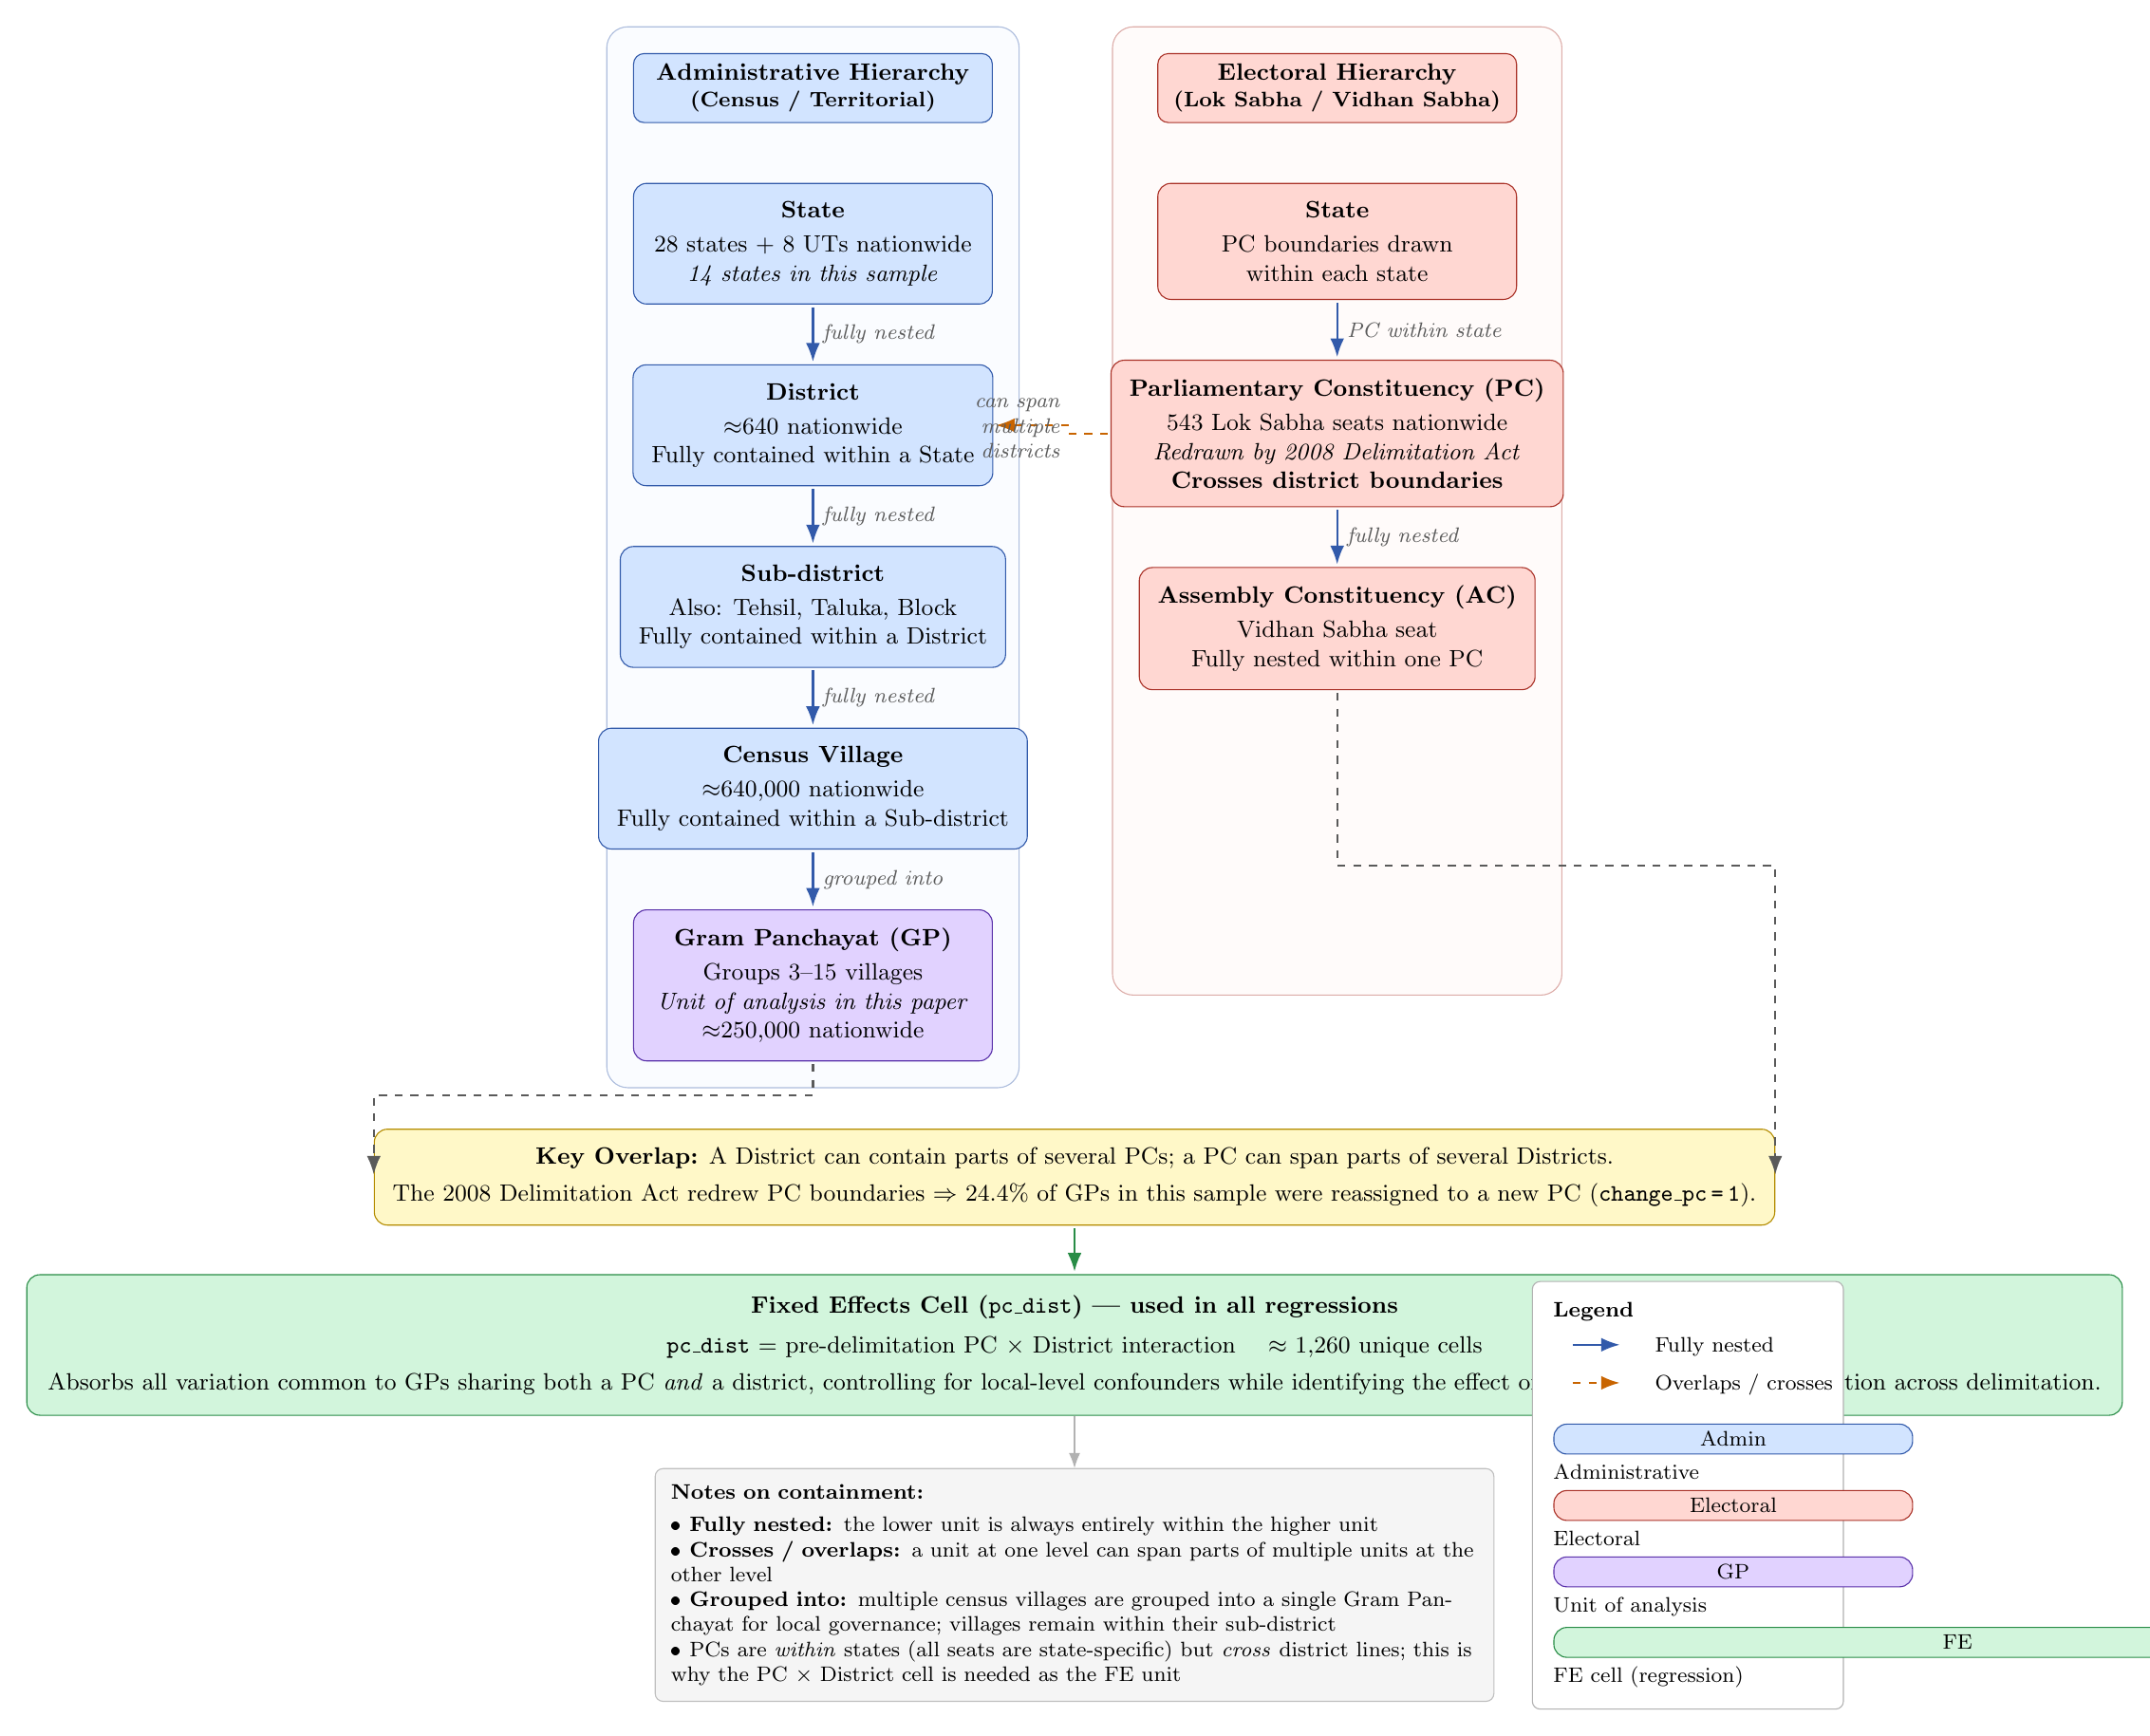
\begin{tikzpicture}[node distance=0.7cm and 1.4cm]

% ══════════════════════════════════════════════════════════════════════════════
% COLUMN HEADERS
% ══════════════════════════════════════════════════════════════════════════════
\node[seclabel, fill=admblue, draw=admborder, rounded corners=4pt,
      minimum width=4.8cm, align=center] (admtitle)
  {\textbf{Administrative Hierarchy}\\[-1pt]{\footnotesize (Census / Territorial)}};

\node[seclabel, fill=elecred, draw=elecborder, rounded corners=4pt,
      minimum width=4.8cm, align=center, right=2.2cm of admtitle] (electitle)
  {\textbf{Electoral Hierarchy}\\[-1pt]{\footnotesize (Lok Sabha / Vidhan Sabha)}};

% ══════════════════════════════════════════════════════════════════════════════
% ADMINISTRATIVE COLUMN
% ══════════════════════════════════════════════════════════════════════════════
\node[admbox, below=0.8cm of admtitle] (state) {%
  \textbf{State}\\[2pt]
  28 states + 8 UTs nationwide\\
  \textit{14 states in this sample}};

\node[admbox, below=0.8cm of state] (district) {%
  \textbf{District}\\[2pt]
  $\approx$640 nationwide\\
  Fully contained within a State};

\node[admbox, below=0.8cm of district] (subdistrict) {%
  \textbf{Sub-district}\\[2pt]
  Also: Tehsil, Taluka, Block\\
  Fully contained within a District};

\node[admbox, below=0.8cm of subdistrict] (village) {%
  \textbf{Census Village}\\[2pt]
  $\approx$640{,}000 nationwide\\
  Fully contained within a Sub-district};

\node[gpbox, below=0.8cm of village] (gp) {%
  \textbf{Gram Panchayat (GP)}\\[2pt]
  Groups 3--15 villages\\
  \textit{Unit of analysis in this paper}\\
  $\approx$250{,}000 nationwide};

% Containment arrows — admin column
\draw[containarrow] (state.south)      -- node[right, bracelab]{fully nested} (district.north);
\draw[containarrow] (district.south)   -- node[right, bracelab]{fully nested} (subdistrict.north);
\draw[containarrow] (subdistrict.south)-- node[right, bracelab]{fully nested} (village.north);
\draw[containarrow] (village.south)    -- node[right, bracelab]{grouped into} (gp.north);

% ══════════════════════════════════════════════════════════════════════════════
% ELECTORAL COLUMN
% ══════════════════════════════════════════════════════════════════════════════
\node[elecbox, below=0.8cm of electitle] (pcstate) {%
  \textbf{State}\\[2pt]
  PC boundaries drawn\\
  within each state};

\node[elecbox, below=0.8cm of pcstate] (pc) {%
  \textbf{Parliamentary Constituency (PC)}\\[2pt]
  543 Lok Sabha seats nationwide\\
  \textit{Redrawn by 2008 Delimitation Act}\\
  \textbf{Crosses district boundaries}};

\node[elecbox, below=0.8cm of pc] (ac) {%
  \textbf{Assembly Constituency (AC)}\\[2pt]
  Vidhan Sabha seat\\
  Fully nested within one PC};

% Containment arrows — electoral column
\draw[containarrow] (pcstate.south) -- node[right, bracelab]{PC within state} (pc.north);
\draw[containarrow] (pc.south) -- node[right, bracelab]{fully nested} (ac.north);

% Gap filler so columns are the same height — invisible placeholders
\node[minimum height=1.1cm, below=0.8cm of ac]    (elecpad1) {};
\node[minimum height=1.1cm, below=0.7cm of elecpad1] (elecpad2) {};

% ══════════════════════════════════════════════════════════════════════════════
% CROSS-COLUMN OVERLAP NOTE
% ══════════════════════════════════════════════════════════════════════════════
% Dashed overlap arrow: PC <-> District
\draw[overlaparrow]
  (pc.west) -- ++(-0.55,0) |- node[pos=0.3, left, bracelab,
    text width=1.8cm, align=right]{can span\\multiple\\districts}
  (district.east);

% ══════════════════════════════════════════════════════════════════════════════
% BOTTOM ROWS — FE cell and overlap summary
% ══════════════════════════════════════════════════════════════════════════════

% Coordinate below both columns
\coordinate (botleft)  at ($(gp.south)!0.5!(gp.south) + (0,-0.8)$);
\coordinate (botright) at ($(elecpad2.south)!0.5!(elecpad2.south)$);
\coordinate (botmid)   at ($(gp.south)!0.5!(elecpad2.south) + (0,-0.9)$);

\node[overlaybox, below=0.9cm of gp, xshift=3.5cm] (overlap) {%
  \textbf{Key Overlap:} A District can contain parts of several PCs; a PC can span parts of
  several Districts.\\[3pt]
  The 2008 Delimitation Act redrew PC boundaries $\Rightarrow$ 24.4\% of GPs in this sample were
  reassigned to a new PC (\texttt{change\_pc\,=\,1}).};

% Arrows from gp and ac into overlap
\draw[overlaparrow, color=annotgrey]
  (gp.south) -- ++(0,-0.45) -| (overlap.west);
\draw[overlaparrow, color=annotgrey]
  (ac.south) -- ++(0,-2.35) -| (overlap.east);

\node[febox, below=0.65cm of overlap] (fecell) {%
  \textbf{Fixed Effects Cell (\texttt{pc\_dist}) — used in all regressions}\\[4pt]
  \texttt{pc\_dist} = pre-delimitation PC $\times$ District interaction
  \quad $\approx$ 1{,}260 unique cells\\[3pt]
  Absorbs all variation common to GPs sharing both a PC \textit{and} a district,
  controlling for local-level confounders while identifying the effect of
  \textit{changes} in political competition across delimitation.};

\draw[containarrow, color=fegreenborder]
  (overlap.south) -- (fecell.north);

% ══════════════════════════════════════════════════════════════════════════════
% NOTES BOX
% ══════════════════════════════════════════════════════════════════════════════
\node[notebox, below=0.7cm of fecell, text width=10.8cm] (notes) {%
  \textbf{Notes on containment:}\\[3pt]
  \textbullet\ \textbf{Fully nested:} the lower unit is always entirely within the higher unit\\
  \textbullet\ \textbf{Crosses / overlaps:} a unit at one level can span parts of multiple units at
  the other level\\
  \textbullet\ \textbf{Grouped into:} multiple census villages are grouped into a single Gram
  Panchayat for local governance; villages remain within their sub-district\\
  \textbullet\ PCs are \textit{within} states (all seats are state-specific) but \textit{cross}
  district lines; this is why the PC $\times$ District cell is needed as the FE unit};

\draw[-{Latex[length=2mm]}, color=black!30] (fecell.south) -- (notes.north);

% ══════════════════════════════════════════════════════════════════════════════
% LEGEND
% ══════════════════════════════════════════════════════════════════════════════
\node[legend, right=0.5cm of notes, yshift=1.2cm, text width=3.6cm] (leg) {%
  \textbf{Legend}\\[4pt]
  \begin{tabular}{cl}
  \tikz\draw[containarrow] (0,0) -- (0.7,0); & Fully nested \\[5pt]
  \tikz\draw[overlaparrow] (0,0) -- (0.7,0); & Overlaps / crosses \\[5pt]
  \end{tabular}\\[4pt]
  \tikz\node[admbox,  text width=1.3cm, minimum height=0.4cm,
             inner sep=2pt, font=\footnotesize]{Admin}; \
  Administrative\\[3pt]
  \tikz\node[elecbox, text width=1.3cm, minimum height=0.4cm,
             inner sep=2pt, font=\footnotesize]{Electoral}; \
  Electoral\\[3pt]
  \tikz\node[gpbox,   text width=1.3cm, minimum height=0.4cm,
             inner sep=2pt, font=\footnotesize]{GP}; \
  Unit of analysis\\[3pt]
  \tikz\node[febox,   text width=1.3cm, minimum height=0.4cm,
             inner sep=2pt, font=\footnotesize]{FE}; \
  FE cell (regression)};

% ══════════════════════════════════════════════════════════════════════════════
% BACKGROUND PANELS for the two columns
% ══════════════════════════════════════════════════════════════════════════════
\begin{pgfonlayer}{background}
  \node[draw=admborder!40, fill=admblue!10, rounded corners=8pt,
        fit=(admtitle)(gp), inner sep=10pt] {};
  \node[draw=elecborder!40, fill=elecred!10, rounded corners=8pt,
        fit=(electitle)(ac)(elecpad1)(elecpad2), inner sep=10pt] {};
\end{pgfonlayer}

\end{tikzpicture}
\end{document}
